\documentclass[UTF8,fontset=windows,11pt]{ctexart}
\usepackage[a4paper,margin=20mm,headheight=15pt]{geometry}
\usepackage{amsmath,amssymb,booktabs,longtable,array,multirow}
\usepackage{siunitx}
\usepackage{xcolor}
\usepackage{tikz}
\usetikzlibrary{arrows.meta,positioning,fit,calc,shapes.geometric,shadows.blur}
\usepackage{adjustbox}
\usepackage{listings}
\usepackage{tcolorbox}
\usepackage{xurl}
\usepackage{hyperref}
\usepackage{fancyhdr}
\usepackage{enumitem}
\usepackage{caption}
\usepackage{pdflscape}
\usepackage{microtype}
\usepackage{seqsplit}

\definecolor{navy}{HTML}{12314A}
\definecolor{teal}{HTML}{087E8B}
\definecolor{cyan}{HTML}{20A4B5}
\definecolor{amber}{HTML}{F2A541}
\definecolor{coral}{HTML}{E85D4A}
\definecolor{green}{HTML}{3D8B63}
\definecolor{paper}{HTML}{F5F1E8}
\definecolor{ink}{HTML}{18222B}
\definecolor{muted}{HTML}{68747D}
\definecolor{verified}{HTML}{DDF4E7}
\definecolor{designed}{HTML}{DCEFFD}
\definecolor{unresolved}{HTML}{FFF0D2}

\hypersetup{
  colorlinks=true,
  linkcolor=navy,
  urlcolor=teal,
  citecolor=green,
  pdftitle={AgInTi C12880MA 高性能固件与 SDK},
  pdfauthor={AgInTi / lazying.art}
}

\pagestyle{fancy}
\fancyhf{}
\lhead{\textcolor{navy}{AgInTi C12880MA Firmware SDK}}
\rhead{\textcolor{muted}{Clean-room Design}}
\cfoot{\thepage}

\setlist[itemize]{leftmargin=2em,itemsep=2pt,topsep=3pt}
\setlist[enumerate]{leftmargin=2.2em,itemsep=3pt,topsep=3pt}
\renewcommand{\arraystretch}{1.25}
\setlength{\parindent}{2em}
\setlength{\parskip}{3pt}
\Urlmuskip=0mu plus 1mu

\lstdefinestyle{code}{
  basicstyle=\ttfamily\small,
  backgroundcolor=\color{paper},
  frame=single,
  rulecolor=\color{muted!40},
  breaklines=true,
  columns=fullflexible,
  showstringspaces=false,
  keywordstyle=\color{teal}\bfseries,
  commentstyle=\color{green},
  stringstyle=\color{coral}
}

\newtcolorbox{verifiedbox}{
  colback=verified,colframe=green,title=已验证（Verified）,fonttitle=\bfseries
}
\newtcolorbox{designbox}{
  colback=designed,colframe=cyan,title={新设计（Designed, not flashed）},fonttitle=\bfseries
}
\newtcolorbox{warningbox}{
  colback=unresolved,colframe=amber,title=尚未硬件验证,fonttitle=\bfseries
}
\newcommand{\code}[1]{\texttt{#1}}

\title{
  \vspace{-1.5cm}
  {\color{navy}\bfseries\LARGE AgInTi C12880MA 高性能固件与 SDK}\\[4pt]
  {\large STM32H743 采集链路逆向理解、clean-room 重构、协议与验证手册}
}
\author{lazying.art}
\date{2026 年 7 月 19 日 \quad 版本 0.2}

\begin{document}
\maketitle

\begin{tcolorbox}[colback=coral!8,colframe=coral,title=安全边界,fonttitle=\bfseries]
本文对应的是一份\textbf{全新编写且仅完成编译验证}的固件。本文生成过程中没有执行
烧录、擦除、解除保护、Option Bytes 写入或 EEPROM 写入。现有 2 MiB 固件镜像能够在
SWD 仍可用时恢复内部应用 Flash，但它不是完整板卡快照；EEPROM 校准、Option Bytes、
OTP 与保护状态仍需在首次烧录前分别只读备份。
\end{tcolorbox}

\begin{abstract}
本报告把 C12880MA 光谱仪控制板的现有接口行为转写为可审计的硬件契约，并据此设计
一套新的 STM32H743 固件、二进制协议与 Python SDK。现有程序的核心瓶颈不是
C12880MA 光敏阵列本身，而是逐边沿 HAL GPIO 调用、逐像素 ADC 轮询、采集与发送串行化，
以及每帧主机请求。新设计使用 TIM2 事件驱动 DMA 写 \code{GPIOE\_BSRR} 产生传感器时钟，
使用 ADC1 外部触发与 DMA 获取 294 个原始样本，并用两个非缓存帧槽把采集和 USB CDC
发送重叠。旧 590 字节协议仍被保留；新 V2 协议增加序号、时间戳、实际曝光、状态、
丢帧计数和 CRC-32。本文明确区分二进制中已经验证的事实、新固件的工程设计，以及必须
通过示波器、稳定光源和对照固件验证的项目。
\end{abstract}

\tableofcontents
\newpage

\section{目标、范围与证据等级}

\subsection{工程目标}

本项目希望在不改变现有 PCB 传感器接线的前提下实现：
\begin{itemize}
  \item 正确复现 C12880MA 的 \code{ST}、\code{CLK}、视频输出采样顺序；
  \item 以确定性硬件时序替代逐边沿函数调用；
  \item 以 DMA 替代逐像素 ADC 轮询；
  \item 采集下一帧时并行发送上一帧，降低帧间死区；
  \item 保留供应商软件所需的旧接口，并提供适合高速流式采集的新接口；
  \item 对每一帧记录足够的可诊断元数据，使高帧率结果可验证而不是只显示一个 FPS；
  \item 在首次烧录前保持原板卡完全不变。
\end{itemize}

\subsection{证据等级}

\begin{longtable}{>{\bfseries}p{0.18\textwidth}p{0.72\textwidth}}
\toprule
等级 & 含义\\
\midrule
\endhead
已验证 & 来自只读 SWD 识别、完整内部 Flash 备份、向量表、反编译控制流、字符串、
工作中的串口/USB 协议，或多个证据彼此一致。\\
官方佐证 & 与 ST 或 Hamamatsu 官方数据手册一致，并能解释二进制行为。\\
新设计 & clean-room 源码已经写出并能够编译，但尚未在目标板运行。\\
待验证 & 必须依赖示波器、逻辑分析仪、稳定光源、暗场或供应商固件对照。\\
\bottomrule
\end{longtable}

\begin{verifiedbox}
当前只读备份 SHA-256 为
\texttt{\seqsplit{67F1F6C421D56C2077D5A3F7417AA6F5213A2791D0C63AE5DAFBDBDF461764B4}}，
大小为 2,097,152 字节。它覆盖 STM32H74x/75x 的 2 MiB 内部 Flash 空间。
\end{verifiedbox}

\section{恢复能力：现在能恢复什么}

\begin{longtable}{p{0.28\textwidth}p{0.16\textwidth}p{0.45\textwidth}}
\toprule
对象 & 当前状态 & 结论\\
\midrule
\endhead
内部 Flash 0x08000000--0x081FFFFF & 已完整备份并哈希 & 在 SWD 可用且保护状态允许时，
可按字节恢复应用代码。\\
外部 I\textsuperscript{2}C EEPROM & 尚未形成独立归档 & 含校正数据；首次烧录前必须通过
现有固件只读导出。已知主要区域至少包括 0x0000--0x0FFF 与 0x1068 附近。\\
Option Bytes / RDP / 启动配置 & 尚未形成清单 & 不属于普通 Flash 镜像；必须读取并记录，
不得盲目写回。\\
OTP 与器件 UID & UID 可读，OTP 未归档 & UID 只用于识别，不应公开；OTP 必须保持只读。\\
系统 Boot ROM & ST 出厂固化 & 不需要也通常不能作为普通应用镜像备份。\\
\bottomrule
\end{longtable}

\begin{warningbox}
因此准确表述是“\textbf{内部 Flash 可恢复}”，不是“整块板已完全可恢复”。只有在 EEPROM、
Option Bytes 和必要 OTP 状态也完成只读归档后，才可以把恢复包称为板卡级备份。
\end{warningbox}

\section{现有固件的硬件契约}

\subsection{引脚与外设}

\begin{table}[htbp]
\centering
\caption{已恢复的信号映射}
\begin{tabular}{lll}
\toprule
功能 & STM32H743 资源 & 证据/说明\\
\midrule
C12880MA ST & PE2 & GPIO 推挽输出\\
C12880MA CLK & PE3 & GPIO 推挽输出；没有可直接使用的定时器输出 AF\\
模拟视频 & PA0 / ADC1\_INP16 & ADC1，单端，16 位配置\\
外部触发 & PE9 / EXTI9\_5 & 上升沿触发采集\\
模式输出 & PE13、PE14 & 由命令模式字节控制\\
校准 EEPROM & PB6/PB7 & 地址 0xA0，16 位存储器地址\\
USB & PB14/PB15 & OTG HS 控制器的 embedded FS PHY\\
\bottomrule
\end{tabular}
\end{table}

\begin{figure}[htbp]
\centering
\begin{adjustbox}{max width=\textwidth}
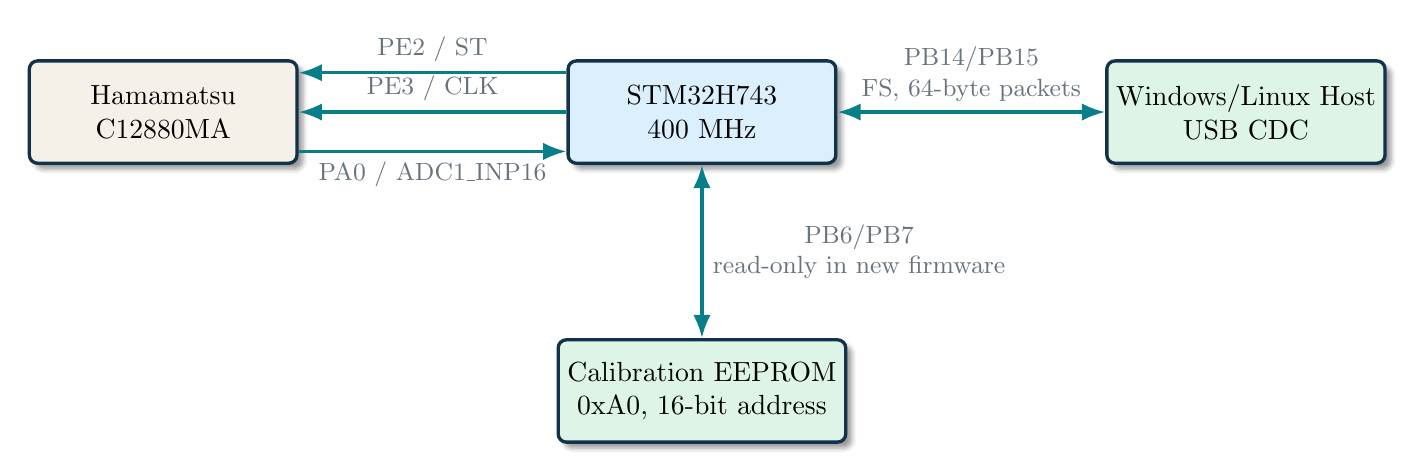
\begin{tikzpicture}[
  >=Latex,
  block/.style={draw=navy,very thick,rounded corners=3pt,fill=white,
                minimum width=34mm,minimum height=13mm,align=center,
                blur shadow},
  bus/.style={->,very thick,color=teal},
  note/.style={font=\small,color=muted,align=center}
]
\node[block,fill=paper] (sensor) {Hamamatsu\\C12880MA};
\node[block,fill=designed,right=34mm of sensor] (mcu) {STM32H743\\400 MHz};
\node[block,fill=verified,right=34mm of mcu] (host) {Windows/Linux Host\\USB CDC};
\node[block,fill=verified,below=22mm of mcu] (eeprom) {Calibration EEPROM\\0xA0, 16-bit address};

\draw[bus] ([yshift=5mm]mcu.west) -- node[above,note]{PE2 / ST} ([yshift=5mm]sensor.east);
\draw[bus] ([yshift=0mm]mcu.west) -- node[above,note]{PE3 / CLK} ([yshift=0mm]sensor.east);
\draw[bus] ([yshift=-5mm]sensor.east) -- node[below,note]{PA0 / ADC1\_INP16} ([yshift=-5mm]mcu.west);
\draw[bus,<->] (mcu) -- node[above,note]{PB14/PB15\\FS, 64-byte packets} (host);
\draw[bus,<->] (mcu) -- node[right,note]{PB6/PB7\\read-only in new firmware} (eeprom);
\end{tikzpicture}
\end{adjustbox}
\caption{控制板的最小硬件模型。箭头方向表示控制或数据方向。}
\end{figure}

\subsection{USB 并不是 USB High-Speed}

现有程序使用 \code{USB\_OTG\_HS} 控制器，但端点最大包长为 64 字节，PHY 配置是
embedded full-speed PHY。STM32H743 若要真正达到 \SI{480}{Mbit/s}，需要外部 ULPI PHY。
因此“使用 HS 控制器”不能等价为“链路在 High-Speed 运行”。新固件保持与现有 PCB 一致
的 Full-Speed 配置。

\subsection{现有采集序列}

二进制控制流给出的顺序如下：
\begin{enumerate}
  \item 清零从 \code{0x24000000} 开始的帧缓冲区；
  \item 输出 12 个预时钟；
  \item PE2（ST）置高；
  \item 输出命令指定数量的积分时钟；
  \item PE2（ST）置低；
  \item 输出 91 个 dummy 时钟；
  \item 对 294 个样本逐个启动 ADC、轮询完成、读数，并在每个样本后输出一个时钟；
  \item 发送 590 字节。
\end{enumerate}

\begin{figure}[htbp]
\centering
\begin{adjustbox}{max width=\textwidth}
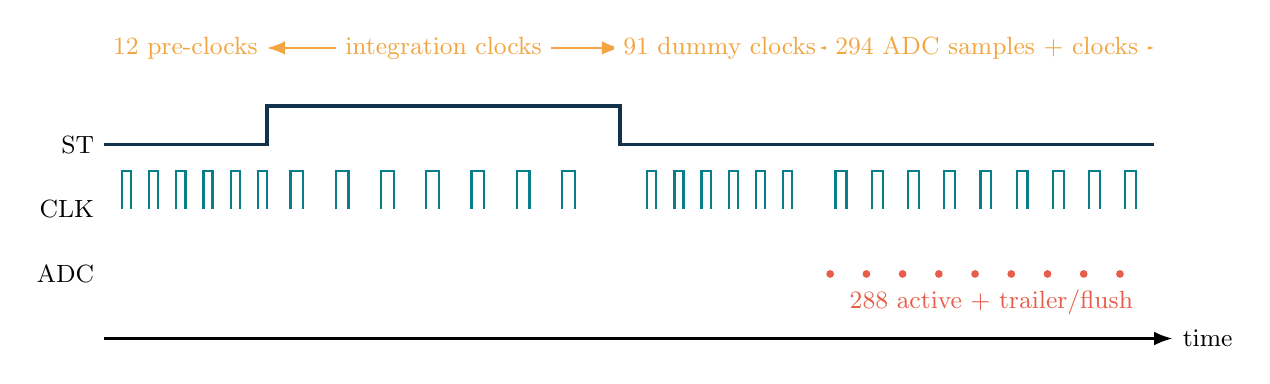
\begin{tikzpicture}[x=0.115cm,y=0.82cm,>=Latex,font=\small]
  \draw[->,thick] (0,0) -- (118,0) node[right]{time};
  \node[left] at (0,3) {ST};
  \node[left] at (0,2) {CLK};
  \node[left] at (0,1) {ADC};
  \draw[navy,very thick] (0,3) -- (18,3) -- (18,3.6) -- (57,3.6) -- (57,3) -- (116,3);
  \foreach \x in {3,6,...,18} {
    \draw[teal,thick] (\x-1,2) -- (\x-1,2.6) -- (\x,2.6) -- (\x,2);
  }
  \foreach \x in {22,27,...,52} {
    \draw[teal,thick] (\x-1.4,2) -- (\x-1.4,2.6) -- (\x,2.6) -- (\x,2);
  }
  \foreach \x in {61,64,...,78} {
    \draw[teal,thick] (\x-1,2) -- (\x-1,2.6) -- (\x,2.6) -- (\x,2);
  }
  \foreach \x in {82,86,...,114} {
    \draw[teal,thick] (\x-1.2,2) -- (\x-1.2,2.6) -- (\x,2.6) -- (\x,2);
    \fill[coral] (\x-1.8,1) circle (1.4pt);
  }
  \draw[<->,amber,thick] (0,4.5) -- node[fill=white]{12 pre-clocks} (18,4.5);
  \draw[<->,amber,thick] (18,4.5) -- node[fill=white]{integration clocks} (57,4.5);
  \draw[<->,amber,thick] (57,4.5) -- node[fill=white]{91 dummy clocks} (79,4.5);
  \draw[<->,amber,thick] (79,4.5) -- node[fill=white]{294 ADC samples + clocks} (116,4.5);
  \node[coral,below] at (98,0.9) {288 active + trailer/flush};
\end{tikzpicture}
\end{adjustbox}
\caption{现有固件的逻辑时序。图中脉冲为分段示意，不按真实脉冲数量绘制。}
\end{figure}

\subsection{590 字节帧的准确含义}

现有代码获取 294 个 16 位 ADC 值，并从帧缓冲区的第 6 个字开始存储。它只发送
295 个字，即：
\[
590\ \mathrm{bytes}
= 6\times2\ \mathrm{header}
+ 288\times2\ \mathrm{active\ pixels}
+ 1\times2\ \mathrm{trailer}.
\]
最后 5 个已经采集的 flush 样本没有通过旧帧发送。V2 协议保留全部 294 个样本，
便于验证读出相位、尾部稳定性和未来算法。

\section{现有性能瓶颈}

\subsection{逐边沿函数调用}

现有程序的传感器时钟并非由定时器输出，而是反复调用 GPIO 写函数。一些脉冲辅助函数
甚至在一个电平上连续调用三次或四次写操作。这会引入函数调用、参数检查、分支和总线
访问开销，也会使边沿间隔依赖编译结果与中断。

\subsection{逐像素 ADC 轮询}

每个样本都经历“启动 ADC、轮询 EOC、读取、停止/下一次”的软件序列。CPU 在转换期间
没有准备下一帧、解析命令或构建 USB 数据。该模式易理解，但不适合作为极限性能路径。

\subsection{串行化的数据路径}

现有主循环近似为
\[
T_{\mathrm{frame,legacy}}
=T_{\mathrm{command}}+T_{\mathrm{capture}}+T_{\mathrm{send}}+T_{\mathrm{wait}}.
\]
新的双缓冲流式设计希望接近
\[
T_{\mathrm{frame,pipeline}}
\approx \max(T_{\mathrm{capture}},T_{\mathrm{send}}),
\]
前提是主机持续读取、USB 队列不阻塞，并且下一帧在空闲帧槽中采集。

\subsection{带宽预算}

旧帧在 \SI{1000}{frame/s} 时的净载荷为
\[
590\times1000=\SI{590}{kB/s}.
\]
旧固件中观察到的 \SI{1.5}{Mbaud} UART，在 8-N-1 下理论净字节率只有
\[
\frac{1.5\times10^6}{10}=\SI{150}{kB/s},
\]
相应帧率上限约为
\[
\frac{150000}{590}\approx254\ \mathrm{frame/s}.
\]
因此 1000 FPS 不可能依赖该 UART。USB Full-Speed CDC/Bulk 在持续读取时具有更高
容量，但 Windows 驱动调度、短包、端点 FIFO 和主机读取粒度都会降低实际吞吐，必须
用序号与丢帧统计实测。

\section{新固件总体结构}

\begin{designbox}
新工程位于 \code{firmware/sdk/}，包含可移植 C 核心、STM32H743 后端、USB CDC、
旧协议兼容层、V2 协议、Python SDK、构建脚本和本文。工程中不存在烧录命令。
\end{designbox}

\begin{figure}[htbp]
\centering
\begin{adjustbox}{max width=\textwidth}
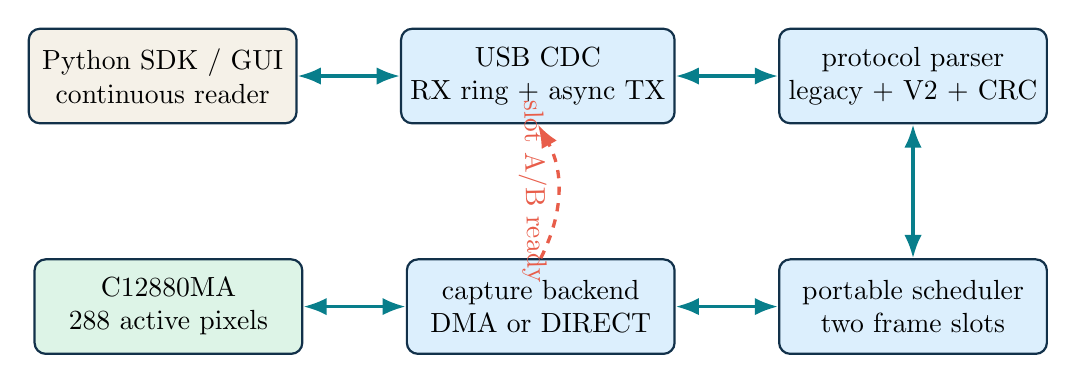
\begin{tikzpicture}[
  >=Latex,
  layer/.style={draw=navy,thick,rounded corners,minimum width=34mm,
                minimum height=12mm,align=center,fill=white},
  flow/.style={->,very thick,teal},
  async/.style={->,very thick,coral,dashed}
]
\node[layer,fill=paper] (host) {Python SDK / GUI\\continuous reader};
\node[layer,fill=designed,right=13mm of host] (usb) {USB CDC\\RX ring + async TX};
\node[layer,fill=designed,right=13mm of usb] (proto) {protocol parser\\legacy + V2 + CRC};
\node[layer,fill=designed,below=17mm of proto] (core) {portable scheduler\\two frame slots};
\node[layer,fill=designed,left=13mm of core] (capture) {capture backend\\DMA or DIRECT};
\node[layer,fill=verified,left=13mm of capture] (sensor) {C12880MA\\288 active pixels};

\draw[flow,<->] (host) -- (usb);
\draw[flow,<->] (usb) -- (proto);
\draw[flow,<->] (proto) -- (core);
\draw[flow,<->] (core) -- (capture);
\draw[flow,<->] (capture) -- (sensor);
\draw[async,bend right=28] (capture.north) to node[below,sloped]{slot A/B ready} (usb.south);
\end{tikzpicture}
\end{adjustbox}
\caption{新固件的软件分层。采集与发送通过帧槽状态而不是共享临时缓冲耦合。}
\end{figure}

\subsection{帧槽状态机}

每个帧槽有四个状态：
\[
\mathrm{FREE}\rightarrow\mathrm{CAPTURING}\rightarrow
\mathrm{READY}\rightarrow\mathrm{TRANSMITTING}\rightarrow\mathrm{FREE}.
\]
只有采集后端写 \code{raw[]}，只有封包阶段写 \code{tx[]}，USB 在
\code{TRANSMITTING} 期间只读 \code{tx[]}。状态转换在短临界区中进行，长时间采集和
USB 传输不关闭中断。

\begin{figure}[htbp]
\centering
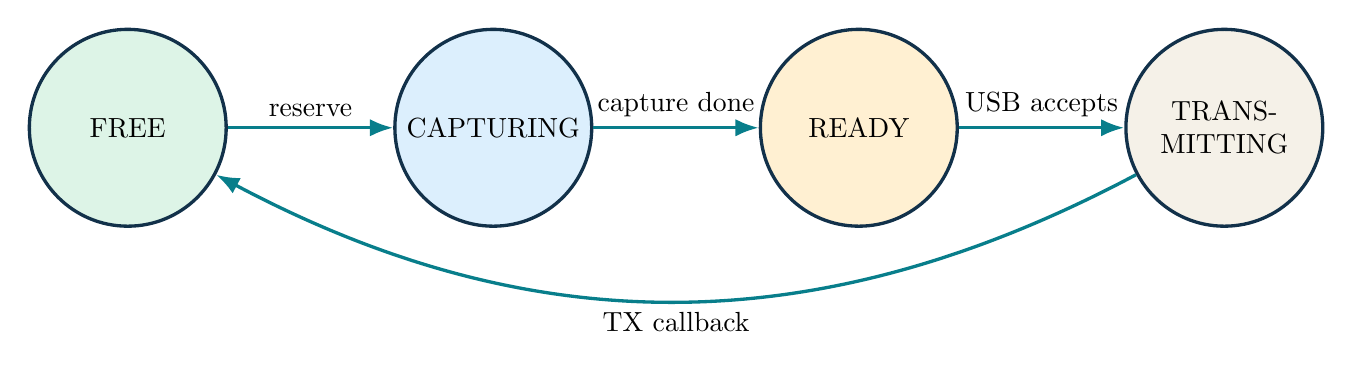
\begin{tikzpicture}[
  >=Latex,node distance=21mm,
  state/.style={draw=navy,very thick,circle,minimum size=25mm,align=center,fill=white},
  every edge/.style={draw=teal,very thick,->}
]
\node[state,fill=verified] (free) {FREE};
\node[state,fill=designed,right=of free] (cap) {CAPTURING};
\node[state,fill=unresolved,right=of cap] (ready) {READY};
\node[state,fill=paper,right=of ready] (tx) {TRANS-\\MITTING};
\path (free) edge node[above]{reserve} (cap)
      (cap) edge node[above]{capture done} (ready)
      (ready) edge node[above]{USB accepts} (tx)
      (tx) edge[bend left=28] node[below]{TX callback} (free);
\end{tikzpicture}
\caption{双缓冲中单个帧槽的生命周期。}
\end{figure}

\subsection{内存与 Cortex-M7 Cache}

STM32H743 的 D-Cache 会造成“CPU 看到新数据但 DMA 看到旧数据”或相反的问题。新固件
把整个设备对象、两个帧槽和 DMA 常量放在 D2 SRAM 的 \code{.dma\_buffer} 段，并用
MPU 把 \code{0x30000000} 起始的 256 KiB 标记为 non-cacheable。这样牺牲少量 CPU
缓存收益，换取清晰且不易遗漏的 DMA 一致性规则。USB PCD 自身关闭 DMA，因此 USB
中间件缓冲不依赖额外 cache clean。

\section{高性能采集后端}

\subsection{为什么不能直接把 PE3 设为定时器 PWM}

STM32H743 数据手册给出的 PE3 复用功能不包含适合输出传感器 CLK 的 TIM 通道。因此在
不改 PCB 的条件下，不能简单执行“TIMx PWM $\rightarrow$ PE3”。本设计把定时器事件
作为 DMA request：
\begin{itemize}
  \item TIM2 Update：DMA1 Stream1 把 \code{GPIO\_PIN\_3} 写入
        \code{GPIOE\_BSRR}，置高 PE3；
  \item TIM2 CH1 Compare：DMA1 Stream2 把
        \code{GPIO\_PIN\_3 << 16} 写入同一 BSRR，置低 PE3；
  \item TIM2 CH2 的内部参考信号：作为 \code{TIM2\_TRGO}，在低电平稳定区触发 ADC1。
\end{itemize}

\begin{figure}[htbp]
\centering
\begin{adjustbox}{max width=\textwidth}
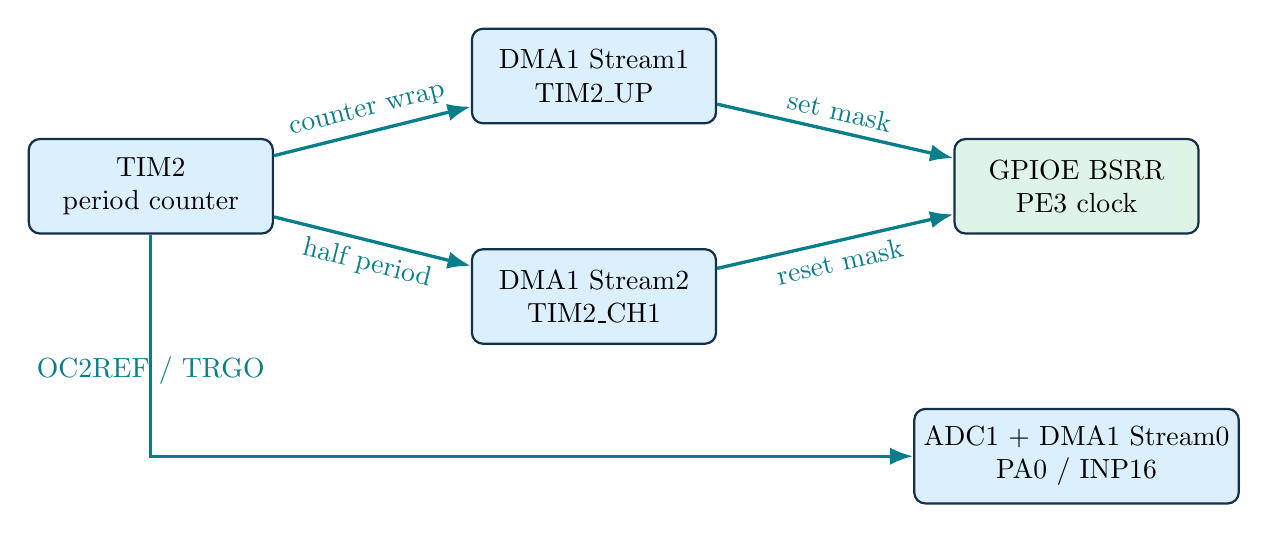
\begin{tikzpicture}[
  >=Latex,
  block/.style={draw=navy,thick,rounded corners,minimum width=31mm,
                minimum height=12mm,align=center,fill=white},
  flow/.style={->,very thick,teal}
]
\node[block,fill=designed] (tim) {TIM2\\period counter};
\node[block,fill=designed,right=25mm of tim,yshift=14mm] (set) {DMA1 Stream1\\TIM2\_UP};
\node[block,fill=designed,right=25mm of tim,yshift=-14mm] (reset) {DMA1 Stream2\\TIM2\_CH1};
\node[block,fill=verified,right=30mm of set,yshift=-14mm] (gpio) {GPIOE BSRR\\PE3 clock};
\node[block,fill=designed,below=22mm of gpio] (adc) {ADC1 + DMA1 Stream0\\PA0 / INP16};

\draw[flow] (tim) -- node[above,sloped]{counter wrap} (set);
\draw[flow] (tim) -- node[below,sloped]{half period} (reset);
\draw[flow] (set) -- node[above,sloped]{set mask} (gpio);
\draw[flow] (reset) -- node[below,sloped]{reset mask} (gpio);
\draw[flow] (tim.south) |- node[below,near start]{OC2REF / TRGO} (adc.west);
\end{tikzpicture}
\end{adjustbox}
\caption{在 PE3 没有定时器输出 AF 时，用定时器触发 DMA 写 BSRR 产生硬件时钟。}
\end{figure}

\subsection{DMA 采样相位}

旧程序是“91 个 dummy clock 后采第一个值，再输出时钟”。新 DMA 方案先输出 90 个
dummy clock，然后启动一个 294 周期的读出段。每个读出周期先产生第 91、92、\ldots
个时钟，在下降沿后的低电平稳定区触发 ADC。这样第一个 ADC 值仍对应第 91 时钟后的
视频输出，且全部 294 点由同一硬件相位获取。

\subsection{积分时间与长曝光}

定义传感器时钟为 $f_{\mathrm{clk}}$，积分时钟数为 $N_{\mathrm{int}}$，则名义积分时间
\[
T_{\mathrm{int}}=\frac{N_{\mathrm{int}}}{f_{\mathrm{clk}}}.
\]
在 \SI{1}{MHz} 下，1 个时钟为 \SI{1}{\micro s}。在 \SI{2}{MHz} 下，1 个时钟为
\SI{0.5}{\micro s}。DMA 的 NDTR 为 16 位；超过 65535 个时钟的曝光被分块。分块之间
会存在很短的软件重启间隔，因此“时钟计数”仍准确，但真实墙钟曝光略长。若需要长曝光
的绝对时间精度，应增加 32 位从定时器门控，而不是把该间隔隐藏。

\subsection{为何默认只设到 1 MHz}

C12880MA 数据手册允许最高 \SI{5}{MHz} CLK，但整个系统还包含 ADC 采样保持与 16 位
转换。ADC 时钟、采样周期、转换周期和模拟前端建立时间必须满足：
\[
T_{\mathrm{sample}}+T_{\mathrm{convert}}+T_{\mathrm{margin}}
<\frac{1}{f_{\mathrm{clk}}}.
\]
把传感器设到 \SI{5}{MHz} 并不自动意味着 16 位 ADC 可以以 \SI{5}{MS/s} 可靠输出。
因此 clean-room 固件默认 \SI{1}{MHz}，软件上限暂定 \SI{2}{MHz}。只有对比暗场噪声、
峰值位置、相邻像素串扰和 ADC overrun 后，才应逐级提高。

\subsection{DIRECT 参考后端}

\code{DIRECT} 后端保留逐样本流程，但直接使用 DWT 周期计数器稳定脉宽。它用于：
\begin{itemize}
  \item 首次确认引脚极性和读出顺序；
  \item 与 DMA 后端进行逐像素差分；
  \item 当 DMA 相位有问题时提供故障隔离基线；
  \item 证明性能提升来自硬件流水而非改变光谱数据语义。
\end{itemize}
它不是性能目标。

\section{协议设计}

\subsection{旧协议}

身份请求为三个字节 \code{04 0D 0A}。兼容采集命令为 9 字节：
\[
\underbrace{\mathrm{FF}}_{\text{start}}\quad
\underbrace{\mathrm{opcode}}_{1}\quad
\underbrace{\mathrm{mode}}_{1}\quad
\underbrace{\mathrm{exposure}}_{4,\ LE}\quad
\mathrm{0D\ 0A}.
\]
正常采集返回固定 590 字节。EEPROM 读命令 0x09 返回 4096 字节，0x10 从 0x1068
附近读取 0x30 字节。为了防止校准被意外破坏，新固件不实现 0x08 和 0x11 的写行为。

\subsection{V2 命令}

\begin{table}[htbp]
\centering
\caption{20 字节 V2 命令头}
\begin{tabular}{rrl}
\toprule
偏移 & 长度 & 字段\\
\midrule
0 & 4 & ASCII \code{ASC2}\\
4 & 1 & 协议版本 2\\
5 & 1 & opcode\\
6 & 2 & flags\\
8 & 4 & sequence\\
12 & 2 & payload length，最大 64\\
14 & 2 & reserved\\
16 & 4 & CRC-32\\
20 & N & payload\\
\bottomrule
\end{tabular}
\end{table}

CRC 使用 IEEE CRC-32，计算时先把 CRC 字段置零。命令支持
\code{HELLO}、\code{GET\_CAPS}、\code{CONFIGURE}、\code{SINGLE\_SHOT}、
\code{START\_STREAM}、\code{STOP\_STREAM}、\code{GET\_STATUS} 和只读
\code{EEPROM\_READ}。

\subsection{V2 光谱帧}

\begin{longtable}{rrp{0.58\textwidth}}
\toprule
偏移 & 长度 & 字段\\
\midrule
\endhead
0 & 4 & ASCII \code{ASP2}\\
4 & 1 & version = 2\\
5 & 1 & header bytes = 48\\
6 & 2 & flags；bit 0 表示 little-endian samples\\
8 & 4 & frame sequence\\
12 & 4 & payload bytes，通常 588\\
16 & 8 & capture-complete timestamp，单位微秒\\
24 & 4 & integration clocks\\
28 & 4 & 实际 sensor clock，单位 Hz\\
32 & 2 & active pixels = 288\\
34 & 2 & raw samples = 294\\
36 & 4 & 状态位，包括 timeout、ADC overrun 与后端类型\\
40 & 4 & 累计 dropped frames\\
44 & 4 & CRC-32\\
48 & 588 & 294 个 little-endian uint16 原始样本\\
\bottomrule
\end{longtable}

序号可以检测丢帧；时间戳可以测量真实帧间隔；状态位可以区分“FPS 看起来高”与
“ADC 已经 overrun”；CRC 可以检测串口缓存错位或不完整帧。

\section{USB、队列与错误恢复}

\subsection{接收路径}

CDC OUT 回调只把字节复制进 1024 字节单生产者/单消费者环形缓冲，并立即重新 arm
端点。命令解析在主循环执行，避免在 USB 中断中进行 EEPROM 访问或启动长采集。
环形缓冲溢出会被计数并通过状态命令公开。

\subsection{发送路径}

帧数据生命周期由帧槽保障。USB 接受缓冲后，帧槽进入 \code{TRANSMITTING}；只有
CDC transmit-complete 回调后才回到 \code{FREE}。控制回复使用单独的 4096 字节缓冲，
且与帧发送互斥。若主机不读数据，采集不会覆盖正在发送的帧。

\subsection{连续流式优于逐帧请求}

逐帧请求会把主机调度延迟叠加到每一帧。V2 的 \code{START\_STREAM} 让设备在两个帧槽
允许的范围内持续采集；主机只需要大块连续读取并按 \code{ASP2} 魔数重同步。停止命令
不擦除数据，也不修改 EEPROM。

\section{EEPROM 的只读策略}

现有 EEPROM 使用 8 位地址 0xA0/0xA1 和 16 位 memory address。新固件用 PB6/PB7
实现低速、开漏、只读软件 I\textsuperscript{2}C，原因是：
\begin{itemize}
  \item 不依赖尚未示波验证的 I2C TIMINGR 常量；
  \item 读取校准发生在停止流式采集后，对吞吐没有影响；
  \item 源码中不存在 EEPROM 写函数，降低误操作风险。
\end{itemize}
首次在板验证时必须确认 SDA/SCL 上拉、电平和 ACK；在此之前“代码编译成功”不能证明
EEPROM 地址或引脚绝对正确。

\section{Python SDK}

Python 包 \code{aginti-c12880} 提供：
\begin{itemize}
  \item V2 命令编码和 CRC；
  \item 增量流解码，可在丢字节后搜索 \code{ASP2} 重同步；
  \item 294 点原始样本和 288 点有效像素视图；
  \item 无后台线程的串行客户端，方便嵌入现有 GUI、Web API 或采集服务；
  \item CLI 身份检测、配置与持续流式 FPS/峰值输出。
\end{itemize}

\begin{lstlisting}[style=code,language=Python]
from aginti_c12880 import SpectrometerClient

with SpectrometerClient("COM7") as dev:
    dev.configure(clock_hz=1_000_000, exposure_clocks=1000)
    dev.start()
    for frame in dev.frames(duration=5.0):
        spectrum = frame.pixels
        print(frame.sequence, frame.timestamp_us, spectrum.max())
    dev.stop()
\end{lstlisting}

\section{构建方法与产物}

\begin{lstlisting}[style=code]
./scripts/fetch_c12880_firmware_deps.ps1
./scripts/build_c12880_firmware.ps1 -Engine DMA -Configuration Release
\end{lstlisting}

依赖脚本固定以下公开源码提交：
\begin{itemize}
  \item STM32H7 HAL：\code{c5e70527126710a6415929ff10c1fd1f40394b1e}；
  \item CMSIS Device H7：\code{de8243d2c15f87936f28a49fcd9e6f5ba10fc233}；
  \item CMSIS 5：\code{55b19837f5703e418ca37894d5745b1dc05e4c91}；
  \item ST USB Device：\code{2df324bd60d4b0bb27404fd70b1c089b467f0e09}。
\end{itemize}

构建生成 ELF、BIN、HEX、MAP，并打印每个文件的 SHA-256。构建脚本没有
\code{openocd}、\code{st-flash}、\code{STM32\_Programmer\_CLI} 或任何 program/erase
动作。

\section{首次烧录前的强制检查}

\begin{enumerate}
  \item 再次核对 2 MiB 固件备份的大小和 SHA-256；
  \item 使用现有供应商固件导出完整 EEPROM，并对导出文件哈希；
  \item 只读记录 Option Bytes、RDP、BOR、boot address、WRP/PCROP；
  \item 记录 MCU 型号、UID 的私有清单，不把 UID 推送到公开仓库；
  \item 准备并人工复核恢复命令，但不要在同一个自动脚本中混合 backup 与 erase；
  \item 明确获得用户“允许烧录”的新指令；
  \item 首次使用 DIRECT 后端和低速 CLK，先验证波形；
  \item 只有 DIRECT 数据与原固件对齐后，再测试 DMA 后端。
\end{enumerate}

\section{首次上板的测量计划}

\subsection{阶段 A：无光学结论的电气验证}

\begin{enumerate}
  \item 示波器通道 1 接 PE2/ST，通道 2 接 PE3/CLK，共地；
  \item 确认复位后 ST、CLK 均为低；
  \item 单帧命令下确认 12 pre-clocks、ST 高宽、dummy/readout 区间；
  \item 检查 CLK 占空比、频率与抖动；
  \item 检查 USB 枚举、身份回复和停止命令；
  \item 不接强光，读取暗场并检查 ADC 是否饱和或全零。
\end{enumerate}

\subsection{阶段 B：数据语义对照}

在同一稳定 LED、光路和积分时间下分别使用供应商固件和新固件采集：
\begin{itemize}
  \item 暗场均值与标准差；
  \item 全 288 像素的逐像素差；
  \item 峰值像素位置；
  \item 总积分强度；
  \item 尾部 6 个 flush/trailer 样本。
\end{itemize}
若光谱整体平移一个像素，应优先检查 dummy clock 和 ADC 触发相位，而不是用软件数组
偏移掩盖。

\subsection{阶段 C：性能阶梯}

建议依次测试 \SI{100}{kHz}、\SI{500}{kHz}、\SI{1}{MHz}、\SI{1.5}{MHz}、
\SI{2}{MHz}。每一档记录：
\[
\mathrm{fps},\quad
\mathrm{sequence\ gaps},\quad
\mathrm{CRC\ errors},\quad
\mathrm{ADC\ overrun},\quad
\mathrm{dark\ noise},\quad
\mathrm{spectral\ RMSE}.
\]
不能只以 FPS 决定“更快”，因为错误采样、重复帧或丢帧也可能显示很高的 UI 刷新率。

\section{性能上限的现实判断}

\subsection{传感器下限}

Hamamatsu 数据手册给出最大 CLK \SI{5}{MHz}，最短扫描周期约
\[
\frac{381}{5\times10^6}=\SI{76.2}{\micro s}.
\]
这说明传感器本身具有远高于当前约 420 FPS 的时间潜力，但实际系统还受到曝光、ADC、
USB、主机和光子噪声限制。

\subsection{1 kFPS 是否可行}

如果一帧为 590 字节，1 kFPS 净载荷为 \SI{590}{kB/s}；V2 帧为 636 字节，
对应 \SI{636}{kB/s}。这处于 USB Full-Speed 可尝试的范围，但并无保证。实现条件至少
包括：
\begin{itemize}
  \item 持续流而非逐帧请求；
  \item 主机串口线程使用足够大的读块；
  \item 设备不在每帧进行 EEPROM、格式化打印或阻塞延时；
  \item ADC 与传感器时钟在目标速率下无 overrun；
  \item 帧序号和 CRC 证明数据真实连续。
\end{itemize}
如果 CDC 驱动成为瓶颈，下一步是自定义 vendor bulk 接口，而不是修改 C12880 时序。

\section{尚未解决的问题}

\begin{warningbox}
以下问题不能从“已编译”得出答案：
\begin{itemize}
  \item PE2/PE3 电平极性在实际 PCB 上是否有额外反相器；
  \item TIM2 CH2 触发相位是否处于模拟视频最佳稳定窗口；
  \item \SI{2}{MHz} 下 16 位 ADC 的 ENOB、串扰和过载裕量；
  \item PB6/PB7 是否与 EEPROM 完全一致，以及软件 I2C 的 ACK；
  \item 供应商主机是否要求身份回复前两个字节的额外语义；
  \item V2 连续流在具体 Windows USB 栈上的稳定吞吐；
  \item 校正 EEPROM 中 4096 字节和 0x1068 区域的精确数据结构。
\end{itemize}
\end{warningbox}

\section{结论}

现有固件已经被理解到足以建立明确的引脚、时序、ADC、USB 和 EEPROM 契约，并识别出
主要性能瓶颈。新的 clean-room 固件把边沿生成、ADC 读出和 USB 发送改造成硬件定时、
DMA 与双缓冲流水线，同时保留旧帧并增加可验证的 V2 元数据。它是一个可编译、可审计、
可逐级验证的候选固件，但在用户明确授权烧录和完成剩余备份之前，它仍然只应作为构建
产物存在。

\section*{主要官方资料}
\begin{itemize}
  \item Hamamatsu C12880MA 产品页：
    \url{https://www.hamamatsu.com/us/en/product/optical-sensors/spectrometers/mini-spectrometer/C12880MA.html}
  \item Hamamatsu C12880MA / C16767MA 数据手册：
    \url{https://www.hamamatsu.com/content/dam/hamamatsu-photonics/sites/documents/99_SALES_LIBRARY/ssd/c12880ma_c16767ma_kacc1226e.pdf}
  \item ST RM0433：
    \url{https://www.st.com/resource/en/reference_manual/rm0433-stm32h743-753-and-stm32h750-value-line-advanced-arm-based-32-bit-mcus-stmicroelectronics.pdf}
  \item STM32H743 数据手册：
    \url{https://www.st.com/resource/en/datasheet/stm32h743vi.pdf}
  \item STM32H7 HAL：
    \url{https://github.com/STMicroelectronics/stm32h7xx-hal-driver}
  \item ST USB Device Middleware：
    \url{https://github.com/STMicroelectronics/stm32-mw-usb-device}
\end{itemize}

\end{document}
